\documentclass[11pt]{article}
\usepackage[utf8]{inputenc}
\usepackage{amsmath, amssymb}
\usepackage{enumitem}
\usepackage{geometry}
\geometry{a4paper, margin=1in}
\usepackage{setspace}
\onehalfspacing
\setlength{\parindent}{0pt}
\setlength{\parskip}{12pt}
\usepackage{tikz}
\usetikzlibrary{calc,shapes.geometric,arrows.meta,positioning,decorations.pathreplacing}
\usepackage{eso-pic}
\usepackage[colorlinks=true,linkcolor=blue,urlcolor=blue,citecolor=blue]{hyperref}
\usepackage{tabularx}
\usepackage{float}
\usepackage{fancyhdr}
\pagestyle{fancy}
\fancyhf{}
\fancyfoot[C]{\small \copyright\ 2026 Marginal Lab}
\renewcommand{\headrulewidth}{0pt}
\renewcommand{\footrulewidth}{0pt}

\AddToShipoutPictureBG{%
  \begin{tikzpicture}[remember picture, overlay]
    \node[rotate=45, scale=7,
          font=\bfseries,
          text=black!8]
      at (current page.center)
      {Marginal Lab};
  \end{tikzpicture}%
}%

\begin{document}

\begin{titlepage}
\AddToShipoutPictureBG*{%
  \AtPageLowerLeft{%
    \begin{tikzpicture}[remember picture, overlay]
      % Grey background
      \fill[gray!25]
        (current page.south west) rectangle (current page.north east);
      % Second-best diagram in lower center
      \begin{scope}[shift={(current page.south)}, yshift=7.5cm]
        \draw[orange!80, line width=1pt, opacity=0.5] (0,0) ellipse (4.5cm and 2.2cm);
        \draw[yellow!80!orange, line width=1pt, opacity=0.5] (0,0) ellipse (2.8cm and 1.4cm);
        \draw[green!70!teal, line width=1pt, opacity=0.5] (0,0) ellipse (1.2cm and 0.6cm);
        \node[star, star points=5, star point ratio=2.2, fill=yellow!80!orange,
              minimum size=10pt, inner sep=0pt] at (0,0) {};
        \node[font=\footnotesize\bfseries, orange!80!black] at (0.9,0.7) {First Best};
        \draw[red!70, line width=2.5pt] (-3.5,-2.8) -- (-3.5,3);
        \draw[red!50, line width=1pt, dashed] (-3.3,-2.5) -- (-3.3,2.8);
        \node[font=\footnotesize\bfseries, red!70!black, rotate=90] at (-3.9,0.5)
          {Constraint};
        \draw[gray!60, line width=1pt, dashed] (0,0) -- (-3.3,0);
        \draw[red!70, line width=1.5pt] (-2,-.15) -- (-1.5,.15);
        \draw[red!70, line width=1.5pt] (-2,.15) -- (-1.5,-.15);
        \node[font=\tiny\bfseries, gray!70] at (-1.7,0.4) {naive};
        \fill[green!70!teal] (-3.5,-0.9) circle (6pt);
        \draw[green!70!teal, line width=1pt, ->, >=stealth] (0,0) -- (-3.4,-0.85);
        \node[font=\footnotesize\bfseries, green!50!black] at (-5.5,-0.9) {Second Best!};
      \end{scope}
    \end{tikzpicture}%
  }%
}%
\vspace*{0.15\textheight}
\begin{center}
{\LARGE\bfseries\textcolor{black}{The Fallacy of Exhaustive Effort:}\\[8pt]
\Large\textcolor{black}{Why Leaving No Stone Unturned Can Bury You}}
\end{center}
\vspace{2em}
\begin{center}
{\Large\textcolor{black}{Marginal Lab}\\[4pt]
\normalsize\url{https://marginallabs.github.io}}
\end{center}
\vspace{0.5em}
\begin{center}
{\large\textcolor{black}{\today}}
\end{center}
\vspace*{\fill}
\thispagestyle{empty}
\end{titlepage}
\setcounter{page}{1}

\begin{abstract}
\noindent
If satisfying all conditions for an optimal outcome is good, then satisfying as many as possible must be second best. This reasoning is false. When a constraint prevents one condition from being met, the remaining conditions are no longer individually desirable. Satisfying them can worsen the outcome. Drawing on the theory of the second best, we show that constrained optima require violating the unconstrained conditions. Doing more of a good thing can push you further from the optimum.
\end{abstract}

\section{The Prevailing Intuition}

We always believe we should \textit{leave no stone unturned} when we pursue our goals. That is, we should do as much as possible to close the gap between the current state and the target. When successful people give lectures, they talk about their ``good'' habits, like sleeping early, waking up early, reading books, and so on. We often treat those people as ``landmarks'' and those habits as \textit{criteria for success}. Therefore, we are sold that we should follow them as much as we can to get close to success. \textit{More effort equals better outcome.}

However, this argument is generally \textbf{not true}. In other words, it is not always preferable to do as much as we can.

\section{The Formal Problem}

Formally, suppose there are \(n\) conditions. Satisfying all of them would lead to a favourable outcome \(X\). Now, given that at least one of the conditions \textit{cannot be satisfied}, should we try our best to satisfy all other conditions? Does this strategy bring us closer to the favourable outcome?

\begin{figure}[ht]
\centering
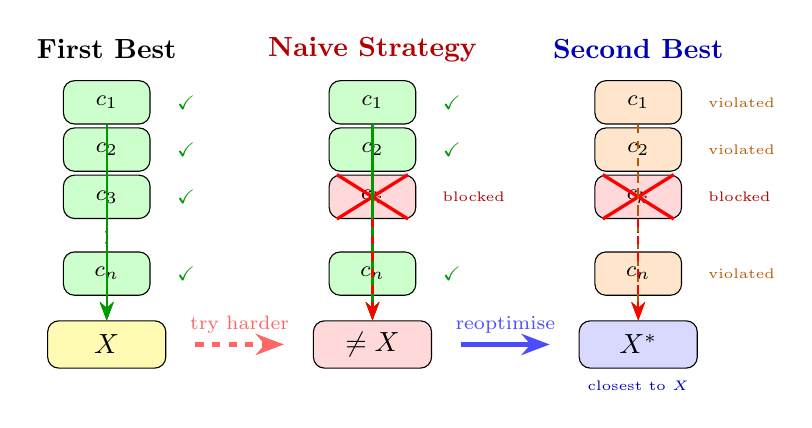
\begin{tikzpicture}[>=Stealth, scale=0.75, every node/.style={font=\footnotesize},
  cond/.style={draw, rounded corners, minimum width=1.1cm, minimum height=0.55cm, inner sep=1pt},
  result/.style={draw, rounded corners, minimum width=1.5cm, minimum height=0.6cm, inner sep=2pt, font=\normalsize\bfseries}]

  % ===== Panel A: First Best (centred at x=0) =====
  \node[font=\normalsize\bfseries] at (0,4) {First Best};

  \node[cond, fill=green!20] (a1) at (0,3.1) {$c_1$};
  \node[cond, fill=green!20] (a2) at (0,2.3) {$c_2$};
  \node[cond, fill=green!20] (a3) at (0,1.5) {$c_3$};
  \node at (0,0.85) {$\vdots$};
  \node[cond, fill=green!20] (aN) at (0,0.2) {$c_n$};

  % Green checks
  \foreach \nd in {a1,a2,a3,aN}
    \node[green!60!black, font=\scriptsize, anchor=west] at ([xshift=8pt]\nd.east) {\checkmark};

  \node[result, fill=yellow!30] (Xa) at (0,-1) {$X$};

  \foreach \nd in {a1,a2,a3,aN}
    \draw[->, thick, green!60!black] (\nd.south) -- (Xa.north);

  % ===== Panel B: Naive Strategy (centred at x=4.5) =====
  \node[font=\normalsize\bfseries, red!70!black] at (4.5,4) {Naive Strategy};

  \node[cond, fill=green!20] (b1) at (4.5,3.1) {$c_1$};
  \node[cond, fill=green!20] (b2) at (4.5,2.3) {$c_2$};
  \node[cond, fill=red!15]    (bk) at (4.5,1.5) {$c_k$};
  \node at (4.5,0.85) {$\vdots$};
  \node[cond, fill=green!20] (bN) at (4.5,0.2) {$c_n$};

  % Checks on unblocked
  \foreach \nd in {b1,b2,bN}
    \node[green!60!black, font=\scriptsize, anchor=west] at ([xshift=8pt]\nd.east) {\checkmark};
  % Cross on blocked
  \draw[red, very thick] ([xshift=-4pt]bk.north east) -- ([xshift=4pt]bk.south west);
  \draw[red, very thick] ([xshift=4pt]bk.north west) -- ([xshift=-4pt]bk.south east);
  \node[red!70!black, font=\tiny, anchor=west] at ([xshift=8pt]bk.east) {blocked};

  \node[result, fill=red!15] (Xb) at (4.5,-1) {$\neq X$};

  \foreach \nd in {b1,b2,bN}
    \draw[->, thick, green!60!black] (\nd.south) -- (Xb.north);
  \draw[->, thick, red, dashed] (bk.south) -- (Xb.north);

  % ===== Panel C: Second Best (centred at x=9) =====
  \node[font=\normalsize\bfseries, blue!70!black] at (9,4) {Second Best};

  \node[cond, fill=orange!20] (c1) at (9,3.1) {$c_1$};
  \node[cond, fill=orange!20] (c2) at (9,2.3) {$c_2$};
  \node[cond, fill=red!15]    (ck) at (9,1.5) {$c_k$};
  \node at (9,0.85) {$\vdots$};
  \node[cond, fill=orange!20] (cN) at (9,0.2) {$c_n$};

  % "violated" labels
  \foreach \nd in {c1,c2,cN}
    \node[orange!70!black, font=\tiny, anchor=west] at ([xshift=8pt]\nd.east) {violated};
  % Cross on blocked
  \draw[red, very thick] ([xshift=-4pt]ck.north east) -- ([xshift=4pt]ck.south west);
  \draw[red, very thick] ([xshift=4pt]ck.north west) -- ([xshift=-4pt]ck.south east);
  \node[red!70!black, font=\tiny, anchor=west] at ([xshift=8pt]ck.east) {blocked};

  \node[result, fill=blue!15] (Xc) at (9,-1) {$X^{*}$};
  \node[blue!70!black, font=\tiny, below=1pt of Xc] {closest to $X$};

  \foreach \nd in {c1,c2,cN}
    \draw[->, thick, orange!70!black, dashed] (\nd.south) -- (Xc.north);
  \draw[->, thick, red, dashed] (ck.south) -- (Xc.north);

  % ===== Comparison arrows between panels =====
  \draw[->, ultra thick, red!60, dashed] (1.5,-1) -- (3,-1)
    node[midway, above, font=\scriptsize] {try harder};
  \draw[->, ultra thick, blue!70] (6,-1) -- (7.5,-1)
    node[midway, above, font=\scriptsize] {reoptimise};

\end{tikzpicture}
\caption{The second-best optimum $X^*$ may require violating the remaining conditions.}
\label{fig:conditions}
\end{figure}

The answer is \textbf{no}. The concept is simple: the optimal strategy depends on your constraints. If you have no constraints, you can satisfy all \(n\) conditions and get a favourable outcome. If you add some constraints to the problem, the objective does not change, but \textit{all} of your optimal conditions are altered because they are often correlated. The optimal solution structure is \textbf{completely different} from the unconstrained problem.

\subsection{The Dinner Party Metaphor}

Imagine you go to a Michelin-starred restaurant. You want to see three things:
\begin{enumerate}[label=(\arabic*)]
    \item Dim lighting.
    \item A big plate with small food.
    \item Nice food.
\end{enumerate}

Now suppose that Condition (3) will not be satisfied. The food is terrible. Would you still want to satisfy Conditions 1 and 2? According to the ``leave no stone unturned'' logic, the answer is yes. You dim the lights romantically. You bring out the giant white plates and arrange the food with tweezers.

But what is the result? You have \textbf{not saved the evening}. You have \textbf{made it worse}. The dim lighting now looks like a deliberate attempt to \textit{hide} the bad food. The large plate makes the small, bad food look even more pathetic by comparison. The whole thing becomes a parody of fine dining. In this scenario, the optimal move is to \textbf{abandon the pretense entirely}: turn on the bright lights and serve the food on a normal plate, or just order pizza.

Of course, this is merely a metaphor to build intuition. Let us now examine some real economic examples.

\subsection{Monopoly and Pollution}

Imagine a society with a monopoly firm that pollutes the water. First, we often say \textit{monopoly is bad}. It is because a monopoly would produce less output than a competitive market and hence set a price higher than that of a competitive market would. It inflicts a loss on the consumers. Second, we often say \textit{pollution is bad}. It is because the firm does not need to pay for the social cost of the pollution, and hence produces more than the optimal amount. It inflicts a loss on society.

\begin{figure}[ht]
\centering
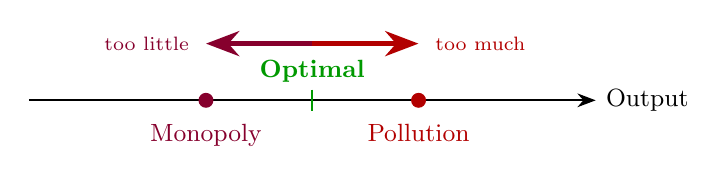
\begin{tikzpicture}[>=Stealth, scale=0.9]
  % Number line
  \draw[thick, ->] (0,0) -- (8,0) node[right, font=\small] {Output};

  % Optimal
  \draw[thick, green!60!black] (4,0.15) -- (4,-0.15);
  \node[green!60!black, above=3pt, font=\small\bfseries] at (4,0) {Optimal};

  % Monopoly (left of optimal)
  \fill[purple!70!black] (2.5,0) circle (3pt);
  \node[purple!70!black, below=5pt, font=\small] at (2.5,0) {Monopoly};
  \draw[<-, line width=2pt, purple!70!black] (2.5,0.8) -- (4,0.8);
  \node[purple!70!black, font=\scriptsize, left] at (2.4,0.8) {too little};

  % Pollution (right of optimal)
  \fill[red!70!black] (5.5,0) circle (3pt);
  \node[red!70!black, below=5pt, font=\small] at (5.5,0) {Pollution};
  \draw[->, line width=2pt, red!70!black] (4,0.8) -- (5.5,0.8);
  \node[red!70!black, font=\scriptsize, right] at (5.6,0.8) {too much};

\end{tikzpicture}
\caption{Monopoly restricts output; pollution expands it.}
\label{fig:monopoly}
\end{figure}

The best policy to handle the problem is, of course, to break up the monopoly and charge a tax on pollution. However, if the monopoly cannot be broken up, or the pollution cannot be measured, what do we do? A piecemeal policy is to ``do as much as we can.'' But it is not optimal in this case.

Breaking up the monopoly increases its production scale and lowers the price, but it means higher pollution. Taxing the pollution means we lower its scale, and hence the price will be even higher. As you may see, the ``bad'' side of monopoly and the ``bad'' side of pollution \textbf{offset each other naturally}. The optimal policy could be \textbf{``do nothing.''}

\subsection{Taxes and Public Goods}

Imagine a society with two ``good'' conditions: \textit{low taxes are good} (they let people keep what they earn and encourage work), and \textit{public goods are good} (roads, courts, defence, you need them). The first-best world satisfies both: the government funds public goods with a lump-sum tax that does not distort anyone's incentives. Everyone works and everyone pays.

Now suppose a lump-sum tax is \textit{not possible}. The government can only raise revenue through income taxes, which distort labour supply. Should we still try to fund public goods as much as we can, because public goods are good? The ``leave no stone unturned'' logic says yes: fund everything, tax everything, do as much as we can.

But this is not optimal. Every additional dollar of income tax discourages work further. At some point, the deadweight loss from taxation outweighs the benefit of the public good it funds. The ``good'' of public goods and the ``good'' of low taxes \textbf{pull against each other}. The optimal policy is not to fund every public good you want. It is to fund only those whose benefit \textit{exceeds} the distortion they cause. Some ``good'' things must be left unfunded, because paying for them makes the overall outcome worse.

\subsection{Flat Taxation and the Leisure Constraint}

You might say: fine, income taxes distort. So let us switch to a \textit{flat general sales tax}. One rate on everything, no exceptions. It sounds simple and it sounds fair. In a world where we could tax \textit{all} goods, it would be optimal.

But here is the catch. A flat sales tax is only optimal if you can tax \textit{all} goods at the same rate. And you cannot. Why? Because \textbf{leisure cannot be taxed}. When someone chooses to work fewer hours and enjoy more free time, the government gets nothing. A parent who stays home to raise children instead of hiring a nanny? That imputed income is invisible to the taxman. A retiree who gardens instead of paying a landscaper? The savings are real, but the tax revenue is gone.

This matters because a flat sales tax makes the choice between consumption and leisure more distorted for some people than others. People who can easily substitute toward home production face a lighter burden than those who cannot. The result? A flat rate raises less revenue from the flexible than a differentiated system would. The second-best optimal commodity tax is \textbf{not} flat. It charges lower rates on goods that compete closely with leisure, precisely because you cannot tax leisure. The ``good'' condition of a uniform rate must be \textbf{violated} to account for the constraint you cannot remove.

\subsection{Summary}

The pattern is the same every time. The ``leave no stone unturned'' logic says: satisfy every good condition you can. But when a constraint binds, satisfying the remaining conditions can make things \textit{worse}. The table below makes this explicit.

\begin{center}
\small
\begin{tabularx}{\textwidth}{|l|X|X|X|}
\hline
\textbf{Example} & \textbf{Believed ``good'' conditions} & \textbf{Reality when a constraint binds} & \textbf{Second-best solution} \\
\hline
Fancy Restaurant & Dim lighting; big plate; nice food & Nice food is impossible. Dim lighting and big plate make bad food look \textit{worse}. & Abandon fine dining. Bright lights, normal plate, or order pizza. \\
\hline
Monopoly \& Pollution & Break up monopoly; tax pollution & One cannot be fixed. Fixing the other amplifies the remaining harm. & Do nothing. The two ``bads'' offset each other. \\
\hline
Taxes \& Public Goods & Low taxes; fund public goods & Lump-sum tax is impossible. Income tax distorts labour supply. & Fund only public goods whose benefit exceeds the distortion. \\
\hline
Flat Sales Tax & Uniform rate on all goods & Leisure cannot be taxed. Flat rate distorts the consumption-leisure choice unevenly. & Differentiate rates. Charge less on goods that compete with leisure. \\
\hline
\end{tabularx}
\end{center}

\section{The Deeper Problem}

\subsection{The Perfectionist Problem}

This intuition does not just sit in your head. It \textbf{demands action}, and that action has a name: the \textit{perfectionist problem}. The perfectionist operates under a harsh rule: If I cannot satisfy all \(n\) conditions perfectly, the whole thing is ruined. \textit{Partial effort is either worthless or even harmful.}

Look at the dinner party example again. The perfectionist, faced with bad food, has two bad options:
\begin{enumerate}
    \item \textbf{Obsessive Overcompensation:} Spend six hours trying to turn microwave lasagna into something fancy. The effort is huge, the result is still bad, and you wasted your whole afternoon.
    \item \textbf{Complete Abandonment:} Cancel the party. ``If it can't be perfect, it can't be at all.'' This is the most common ending. By insisting on a 10 out of 10, you settle for a 0 out of 10 when a solid 7 was sitting right there.
\end{enumerate}

The perfectionist forgets that the \textbf{objective function has changed}. The question is no longer ``How do I have the perfect French dinner?'' It is now \textit{``Given the food is bad, what is the best evening I can still make?''} The answer to that new question often requires \textbf{throwing out the old landmark criteria completely}.

\subsection{The Fallacy of Misplaced Valuation}

You may say I am being consequentialist, and maybe that is right. We should always judge the \textbf{outcome}, not the individual conditions.

``Being successful is good'' is our \textit{value judgement}. ``Waking up early, reading books will make you successful'' is a \textit{factual statement}. We should not confuse the logical consequences and incorrectly impose value judgements on the conditions.

The thinking fallacy is exactly this. Because we want the outcome (success), we start to believe that the \textbf{conditions themselves are morally good}. We start to say ``waking up early is a virtue'' instead of ``waking up early is a useful tool.'' We treat the landmark as if it were the \textit{destination itself}.

But it gets worse. The fallacy \textbf{flips the reasoning entirely}. Instead of asking ``What does this outcome actually require?'', you start asking ``What outcome do these conditions guarantee?'' The first question works backward from the goal. The second just hopes the goal somehow follows from the means. The conditions of success are \textit{neither necessary nor sufficient}. Mix them up, and practical wisdom becomes dogma.

And that is why the fallacy is so hard to shake. When someone points out that a condition is not working, you do not question the condition, you question the \textit{effort}. ``You must not be trying hard enough.'' The condition itself is never up for debate, because you have turned it from a useful observation into a moral truth.

\begin{figure}[H]
\centering
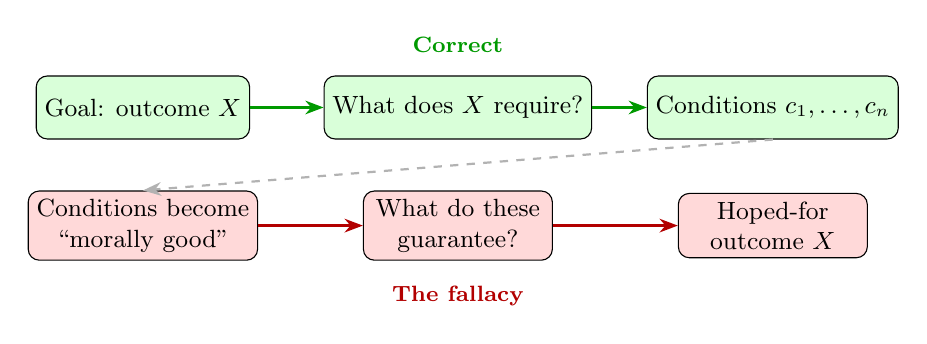
\begin{tikzpicture}[>=Stealth, every node/.style={font=\small},
  box/.style={draw, rounded corners, minimum width=2.4cm, minimum height=0.8cm, align=center, inner sep=3pt}]

  % Top row: Correct reasoning
  \node[box, fill=green!15] (goal) at (0,1.5) {Goal: outcome $X$};
  \node[box, fill=green!15] (ask1) at (4,1.5) {What does $X$ require?};
  \node[box, fill=green!15] (cond1) at (8,1.5) {Conditions $c_1, \ldots, c_n$};
  \draw[->, thick, green!60!black] (goal) -- (ask1);
  \draw[->, thick, green!60!black] (ask1) -- (cond1);
  \node[green!60!black, font=\footnotesize\bfseries] at (4,2.3) {Correct};

  % Bottom row: The fallacy
  \node[box, fill=red!15] (cond2) at (0,0) {Conditions become\\``morally good''};
  \node[box, fill=red!15] (ask2) at (4,0) {What do these\\guarantee?};
  \node[box, fill=red!15] (goal2) at (8,0) {Hoped-for\\outcome $X$};
  \draw[->, thick, red!70!black] (cond2) -- (ask2);
  \draw[->, thick, red!70!black] (ask2) -- (goal2);
  \node[red!70!black, font=\footnotesize\bfseries] at (4,-0.9) {The fallacy};

  % Arrow connecting top to bottom
  \draw[->, thick, gray!60, dashed] (cond1.south) -- (cond2.north);
\end{tikzpicture}
\caption{The fallacy flips the reasoning direction.}
\label{fig:fallacy}
\end{figure}

\section{Conclusion}

The right strategy depends on your constraints. No constraints? Satisfy every condition and enjoy the outcome. But constraints are usually binding, and when they are, you cannot just copy the habits of the landmark people and hope for the best. The optimal solution is \textbf{completely different}. Sometimes, doing less of a good thing is the only way to keep the whole thing from falling apart. Sometimes, the stone you leave unturned is the one that was going to bury you.

\appendix
\section*{Appendix}
\addcontentsline{toc}{section}{Appendix}
\subsection*{The Theory of the Second Best}

The theory of the second best, introduced by Lipsey and Lancaster (1956), addresses a fundamental question in welfare economics: if one of the conditions required for a \textit{Pareto-optimal} allocation cannot be satisfied, what is the best attainable outcome? The intuitive answer, satisfying as many of the remaining conditions as possible, is \textbf{formally incorrect}.

Consider a general equilibrium system characterised by \(n\) first-order conditions for optimality. When all \(n\) conditions hold simultaneously, the system achieves a \textit{first-best optimum}. Now suppose a constraint prevents condition \(i\) from being satisfied, so that the system deviates from the optimum along dimension \(i\). Lipsey and Lancaster demonstrated that the new optimum (the ``second best'') generally requires violating \textbf{all} of the remaining \(n - 1\) conditions as well. The reason is that the first-order conditions are typically \textit{interdependent}: they are derived from a system of simultaneous equations, so perturbing one condition alters the marginal trade-offs throughout the entire system.

The key insight is that \textit{piecemeal welfare policy}, attempting to move ``closer'' to the first-best by satisfying individual conditions in isolation, \textbf{can reduce welfare relative to doing nothing at all}. The theory thus provides a formal justification for \textbf{holistic}, rather than incremental, policy design in second-best environments.

\subsection*{Proof via Lagrange Multipliers}

Let the objective function be \(F(x_1, x_2, \ldots, x_n)\) subject to the optimality conditions
\[
  g_k(x_1, x_2, \ldots, x_n) = 0, \quad k = 1, 2, \ldots, n.
\]

\textbf{First-best.} At the unconstrained optimum, all \(n\) conditions hold. The Lagrangian is
\[
  \mathcal{L} = F(x_1, \ldots, x_n) + \sum_{k=1}^{n} \lambda_k \, g_k(x_1, \ldots, x_n),
\]
and the first-order conditions are
\[
  \frac{\partial F}{\partial x_i} + \sum_{k=1}^{n} \lambda_k \frac{\partial g_k}{\partial x_i} = 0, \quad i = 1, 2, \ldots, n. \tag{1}
\]
This is a system of \(n\) equations in \(n\) unknowns \((x_1, \ldots, x_n)\) with \(n\) multipliers \((\lambda_1, \ldots, \lambda_n)\). Denote the first-best solution by \((\bar{x}_1, \ldots, \bar{x}_n)\) with multipliers \((\bar{\lambda}_1, \ldots, \bar{\lambda}_n)\).

\textbf{Second-best.} Now suppose a constraint forces the system to violate condition \(i\): \(g_i(x_1, \ldots, x_n) = c \neq 0\). The remaining \(n - 1\) conditions \(g_k = 0\) for \(k \neq i\) are still available. The new Lagrangian is
\[
  \mathcal{L}' = F(x_1, \ldots, x_n) + \mu_i\,(g_i - c) + \sum_{k \neq i} \mu_k \, g_k(x_1, \ldots, x_n),
\]
where the constraint \(g_i = c\) is now explicit. The new first-order conditions are
\[
  \frac{\partial F}{\partial x_j} + \mu_i \frac{\partial g_i}{\partial x_j} + \sum_{k \neq i} \mu_k \frac{\partial g_k}{\partial x_j} = 0, \quad j = 1, 2, \ldots, n. \tag{2}
\]

\textbf{Step 1: The multipliers change.} Compare (1) and (2). They share the same left-hand side \(\partial F / \partial x_j\), so
\[
  \sum_{k=1}^{n} \lambda_k \frac{\partial g_k}{\partial x_j} = \mu_i \frac{\partial g_i}{\partial x_j} + \sum_{k \neq i} \mu_k \frac{\partial g_k}{\partial x_j}, \quad j = 1, \ldots, n.
\]
This is a system of \(n\) linear equations in the multipliers. The first-best multipliers \((\bar{\lambda}_1, \ldots, \bar{\lambda}_n)\) satisfy the version evaluated at \((\bar{x}_1, \ldots, \bar{x}_n)\). But the second-best solution \((x_1^*, \ldots, x_n^*)\) must satisfy the constraint \(g_i = c\), so in general \(x^* \neq \bar{x}\). Since the partial derivatives \(\partial g_k / \partial x_j\) are evaluated at a different point and the constraint \(g_i = c\) imposes a different feasible set, the system for the \(\mu_k\) is different from the system for the \(\lambda_k\). Therefore \(\mu_k \neq \bar{\lambda}_k\) in general.

\textbf{Step 2: The optimal values of \(x\) change.} For any \(j\), the second-best condition (2) gives
\[
  \frac{\partial F}{\partial x_j} = -\sum_{k=1}^{n} \mu_k \frac{\partial g_k}{\partial x_j},
\]
which depends on \textit{every} \(\mu_k\), including \(\mu_i\). Since \(\mu_i \neq \bar{\lambda}_i\), the right-hand side differs from the first-best condition for every \(j\), not just \(j = i\). Therefore every optimal \(x_j^*\) generally differs from \(\bar{x}_j\).

\textbf{Step 3: The remaining conditions are violated.} This is the crucial step. The theorem does not merely claim that the multipliers and optimal values change. It claims that at the second-best optimum, the remaining optimality conditions \(g_k(x^*) = 0\) for \(k \neq i\) are \textit{themselves violated}.

Suppose for contradiction that some condition \(g_m(x^*) = 0\) for \(m \neq i\) still holds at the second-best optimum. Then the constraint \(g_m = 0\) is slack at \(x^*\), which means the complementary slackness condition implies \(\mu_m = 0\). But the first-best multiplier \(\bar{\lambda}_m\) is generally nonzero (the constraint \(g_m = 0\) binds at the first-best). So \(\mu_m = 0 \neq \bar{\lambda}_m\). This change in \(\mu_m\) propagates through every equation in (2), shifting the optimal values of all other variables. Since the system is interdependent, this shift will generally cause other constraints \(g_k\) for \(k \neq i, m\) to move away from zero as well. The only way to satisfy all \(g_k(x^*) = 0\) for \(k \neq i\) would be to recover the first-best solution \(\bar{x}\), which violates \(g_i = c\). Contradiction.

Therefore, when one optimality condition cannot be satisfied, the second-best solution generally requires violating \textbf{all} remaining conditions as well.

\section*{References}

\noindent Lipsey, R.\,G., \& Lancaster, K. (1956). The general theory of second best. \textit{The Review of Economic Studies}, \textit{24}(1), 11--32. \url{https://doi.org/10.2307/2296233}

\end{document}